%Este trabalho está licenciado sob a Licença Atribuição-CompartilhaIgual 4.0 Internacional Creative Commons. Para visualizar uma cópia desta licença, visite http://creativecommons.org/licenses/by-sa/4.0/deed.pt_BR ou mande uma carta para Creative Commons, PO Box 1866, Mountain View, CA 94042, USA.

\chapter{Integração}\label{cap_int}
\thispagestyle{fancy}

\ifispython
\begin{obs}\label{obs:cap_int_python}
  Nos códigos \verb+Python+ apresentados neste capítulo, assumimos o seguinte preâmbulo:
\begin{verbatim}
from sympy import *
var('x',real=True)
\end{verbatim}
\end{obs}
\fi

\section{Noção de integral}\label{cap_int_sec_nocaoint}

\subsection{Soma de Riemann}

Seja $f$ uma função contínua definida em um intervalo fechado $[a, b]$. Seja, também, $P$ a seguinte \emph{partição} de $[a, b]$
\begin{equation}
  P = \{a=x_0<x_1<x_2<\cdots<x_n=b\},
\end{equation}
onde $n+1$ é o número de pontos na partição. Definimos
\begin{equation}
  \Delta x_i = x_{i} - x_{i-1}
\end{equation}
o tamanho de cada subintervalo $I_{i} = [x_{i-1}, x_{i}]$ da partição, com $i = 1, 2, \cdots, n$. A \emph{norma da partição} é definida por
\begin{equation}
  \|P\| = \max_{i=1, \dotsc, n} \Delta x_i,
\end{equation}
i.e. o tamanho do maior subintervalo da partição. Com isso, chama-se de uma \emph{soma de Riemann} toda a expressão da forma
\begin{equation}
  S_n := \sum_{i=1}^n f(x_i^*)\Delta x_i,
\end{equation}
onde $x_i^*\in [x_i, x_{i-1}]$ (arbitrariamente escolhido).

\begin{figure}[H]
  \centering
  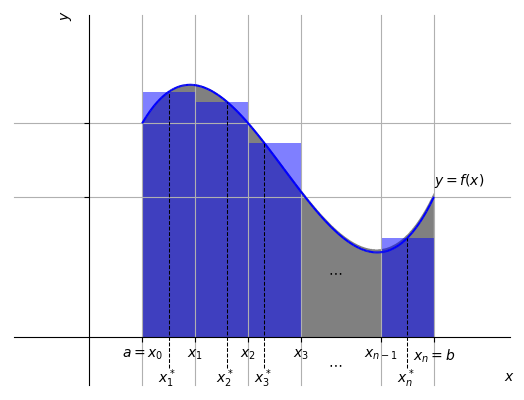
\includegraphics[width=0.9\textwidth]{./cap_int/dados/fig_soma_de_Riemann/fig_soma_de_Riemann}
  \caption{Ilustração da soma de Riemann.}
  \label{fig:soma_de_Riemann}
\end{figure}

\begin{obs}\normalfont{(Aproximação da área sob o gráfico)}
No caso de uma função não negativa, uma soma de Riemann é uma aproximação da área sob seu gráfico e o eixo das abscissas\footnote{Veja o Exercício \ref{exer:int_geoRiemann} para uma interpretação geométrica no caso geral de funções contínuas.}. Veja a Figura \ref{fig:soma_de_Riemann}.
\end{obs}

\subsection{Integral}

A integral (definida) de $a$ até $b$ de uma dada função $f$ em relação a $x$ é denotada e definida por
\begin{equation}
  \int_a^b f(x)\,dx := \lim_{\|P\|\to 0} \sum_{i=1}^n f(x_i^*)\Delta x_i.
\end{equation}
De forma genérica, a integral definida de $a$ até $b$ é o limite das somas de Riemann quando a norma das partições $P$ do intervalo $[a, b]$ tendem a zero. Quando o limite existe, dizemos que $f$ é \emph{integrável} no intervalo $[a, b]$.

\begin{obs}
  Na notação de integral definida acima, chamamos $a$ de \emph{limite inferior} e $b$ de \emph{limite superior de integração}, $f$ é chamada de \emph{integrando} e $x$ de \emph{variável de integração}.
\end{obs}

\begin{obs}
  Funções contínuas são funções integráveis.
\end{obs}

\begin{figure}[H]
  \centering
  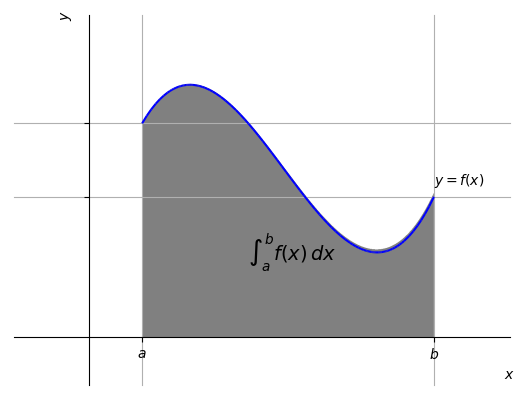
\includegraphics[width=0.9\textwidth]{./cap_int/dados/fig_geointdef/fig_geointdef}
  \caption{A integral definida como a área sob o gráfico.}
  \label{fig:geointdef}
\end{figure}

\begin{obs}\normalfont{(Área sob o gráfico)}\label{obs:int_area}
  No caso de uma função não negativa,
  \begin{equation}
    \int_a^b f(x)\,dx
  \end{equation}
  é a área sob o gráfico de $f$\footnote{Veja o Exercício \ref{exer:int_geointdef} para uma interpretação geométrica no caso geral de funções contínuas.}. Veja a Figura \ref{fig:geointdef}.  
\end{obs}

\begin{ex}
  Vamos calcular
  \begin{equation}
    \int_0^1 1\,dx.
  \end{equation}
  Aqui, o integrando é a função constante $f(x) \equiv 1$ e o \emph{intervalo de integração} é $[a, b]$. Da Observação \ref{obs:int_area}, temos que esta integral é a área sob o gráfico de $f$ no intervalo $[0, 1]$. Esta área é um retângulo de altura $1$ e comprimento $1$. Logo,
  \begin{equation}
    \int_0^1 1\,dx = 1\cdot 1 = 1.
  \end{equation}
\end{ex}

\subsection*{Exercícios resolvidos}

\begin{exeresol}
  Calcule
  \begin{equation}
    \int_{-1}^1 \sqrt{1 - x^2}\,dx.
  \end{equation}
\end{exeresol}
\begin{resol}
  Esta integral corresponde à área sob o gráfico da função $f(x) = \sqrt{1 - x^2}$ restrita ao intervalo $[-1, 1]$. Observando que
  \begin{align}
    y = \sqrt{x^2 - 1} &\Rightarrow y^2 = 1 - x^2\\
                       &\Rightarrow y^2 + x^2 = 1,
  \end{align}
  vemos que esta é a área do semicírculo de raio $1$. Logo,
  \begin{equation}
    \int_{-1}^1 \sqrt{1 - x^2}\,dx = \frac{\pi \cdot 1^2}{2} = \frac{\pi}{2}.
  \end{equation}
\end{resol}

\begin{exeresol}
  Determine a função $F(x)$ tal que
  \begin{equation}
    F(x) = \int_0^x t\,dt,
  \end{equation}
  para todo $x\geq 0$. Então, mostre que $F'(x) = x$.
\end{exeresol}
\begin{resp}
  A integral definida
  \begin{equation}
    \int_0^x t\,dt
  \end{equation}
  é a área sob o gráfico de $f(t) = t$ restrita no intervalo $[0, x]$. Isto é, a área do triângulo retângulo de base $x$ e altura $x$. Logo,
  \begin{equation}
    F(x) = \int_0^x t\,dt = \frac{x\cdot x}{2} = \frac{x^2}{2}.
  \end{equation}
  Ou seja, temos $F(x) = x^2/2$ e, portanto,
  \begin{equation}
    F'(x) = \frac{1}{2}\cdot 2x = x.
  \end{equation}
\end{resp}

\subsection*{Exercícios}

\begin{exer}
  Calcule
  \begin{equation}
    \int_{-1}^2 2\,dx.
  \end{equation}
\end{exer}
\begin{resp}
  $6$
\end{resp}

\begin{exer}
  Calcule
  \begin{equation}
    \int_{-3}^{-1} 1-x\,dx.
  \end{equation}
\end{exer}
\begin{resp}
  $6$
\end{resp}

\begin{exer}
  Determine $F(x)$ tal que
  \begin{equation}
    F(x) = \int_{0}^{x} t+1\,dt.
  \end{equation}
  para $x\geq 0$. Então, calcule $F'(x)$.
\end{exer}
\begin{resp}
  $\displaystyle F(x) = \frac{x^2}{2} + x$; $F'(x) = x + 1$.
\end{resp}

\begin{exer}\label{exer:int_geoRiemann}
  Faça uma interpretação geométrica da uma soma de Riemann aplicada a uma função contínua e não positiva. Estenda sua interpretação para funções contínuas arbitrárias.
\end{exer}
\begin{resp}
  Dica: a soma de Riemann é uma aproximação da área líquida sob o gráfico da função.
\end{resp}

\begin{exer}\label{exer:int_geointdef}
  Faça uma interpretação geométrica de
  \begin{equation}
    \int_a^b f(x)\,dx
  \end{equation}
  quando $f$ é uma função contínua e não positiva. Estenda sua interpretação para funções contínuas arbitrárias.
\end{exer}
\begin{resp}
  Dica: $\displaystyle \int_a^b f(x)\,dx$é a área líquida sob o gráfico da função.
\end{resp}

\begin{exer}
  Calcule
  \begin{equation}
    \int_{-1}^2 -1\,dx.
  \end{equation}
\end{exer}
\begin{resp}
  $-3$
\end{resp}

\begin{exer}
  Calcule
  \begin{equation}
    \int_{-1}^{1} x\,dx.
  \end{equation}
\end{exer}
\begin{resp}
  $0$
\end{resp}

\section{Propriedades de integração}\label{cap_int_sec_propint}

Na Seção \ref{cap_int_sec_nocaoint}, vimos que a integral definida de uma dada função $f$ em um intervalo $[a, b]$ está associada à área (líquida) entre seu gráfico e as retas $y=0$, $x=a$ e $x=b$. Veja a Figura \ref{fig:geointdef}.

Com base nesta noção geométrica, podemos inferir as seguintes propriedades de integração para funções integráveis $f$ e $g$:
\begin{enumerate}[a)]
\item $\displaystyle \int_a^a f(x)\,dx = 0$
\item $\displaystyle \int_a^b k\cdot f(x)\,dx = k\cdot\int_a^b f(x)\,dx$
\item $\displaystyle \int_a^b \left[f(x)\pm g(x)\right]\,dx = \int_a^b f(x)\,dx \pm \int_a^b g(x)\,dx$
\item $\displaystyle \int_a^b f(x)\,dx = \int_a^c f(x)\,dx + \int_c^b f(x)\,dx$
\item $\displaystyle \min_{x\in [a, b]} \{f(x)\}\cdot (b-a) \leq \int_a^b f(x)\,dx \leq \max_{x\in [a, b]} \{f(x)\}\cdot (b-a)$
\end{enumerate}

\begin{ex}
  Sejam $f$ e $g$ funções integráveis tais que
  \begin{align}
    \int_{-1}^4 f(x)\,dx = 2,\\
    \int_4^5 f(x)\,dx = 3,\\
    \int_{-1}^4 g(x)\,dx = -1.
  \end{align}
  Então, vejamos os seguintes casos:
  \begin{enumerate}[a)]
  \item
    \begin{equation}
      \int_{4}^{-1} g(x)\,dx = -\int_{-1}^4 g(x)\,dx = -(-1) = 1.
    \end{equation}
  \item
    \begin{equation}
      \int_{-1}^{-1} 4f(x)\,dx = 0.
    \end{equation}
  \item
    \begin{equation}
      \int_{-1}^{4} -2g(x)\,dx = -2\int_{-1}^4 g(x)\,dx = 2.
    \end{equation}
  \item
    \begin{align}
      \int_{-1}^{4} \left[f(x) - 2g(x)\right]\,dx &= \int_{-1}^{4} f(x)\,dx - \int_{-1}^4 2g(x)\,dx \\
                                                  &= 2 - 2\int_{-1}^4 g(x)\,dx \\
                                                  &= 2 + 2 = 4.
    \end{align}
  \item
    \begin{align}
      \int_{-1}^5 f(x)\,dx &= \int_{-1}^4 f(x)\,dx + \int_{4}^5 f(x)\,dx \\
                           &= 2 + 3 = 5.
    \end{align}
  \end{enumerate}
\end{ex}

\begin{ex}
  Lembrando que $-1 \leq \sen x \leq 1$, temos da propriedade e) acima que
  \begin{align}
    &2\pi \min_{x\in [-\pi, \pi]} \{\sen(x)\} \leq \int_{-\pi}^\pi \sen(x)\,dx \leq 2\pi \max_{x\in [\-pi, \pi]} \{\sen(x)\} \\
    &\Rightarrow -2\pi \leq \int_{-\pi}^\pi \sen(x)\,dx \leq 2\pi.
  \end{align}
\end{ex}

\subsection{Teorema do valor médio}

Com base na noção de integral, define-se a média de uma função $f$ no intervalo $[a, b]$ por
\begin{equation}
  \frac{1}{b-a}\int_a^b f(x)\,dx,
\end{equation}
no caso de $f$ ser integrável neste intervalo.

\begin{teo}\normalfont{(Teorema do valor médio para integrais)}\label{teo:int_teomed}
  Se $f$ for contínua em $[a, b]$, então existe $c\in [a, b]$ tal que
  \begin{equation}
    f(c) = \frac{1}{b-a}\int_a^b f(x)\,dx.
  \end{equation}
\end{teo}
\begin{dem}
  Vejamos uma ideia da demonstração. Da propriedade de integração e) acima, temos
  \begin{equation}
    \min_{x\in [a, b]} \{f(x)\} \leq \frac{1}{b-a}\int_a^b f(x)\,dx \leq \max_{x\in [a, b]} \{f(x)\}.
  \end{equation}
  Agora, pelo Teorema do valor intermediário (Teorema \ref{teo:valorintermediario}), temos $f$ assume todos os valores entre seus valores mínimo e máximo. Logo, existe $c\in [a, b]$ tal que
  \begin{equation}
    f(c) = \frac{1}{b-a}\int_a^b f(x)\,dx.
  \end{equation}  
\end{dem}

\begin{ex}
  Seja $f$ uma função contínua em $[a, b]$, $a\neq b$, e
  \begin{equation}
    \int_a^b f(x)\,dx = 0,
  \end{equation}
  então $f$ possui pelo menos um zero neste intervalo. De fato, do Teorema do valor médio para integrais, temos que existe $c\in [a, b]$ tal que
  \begin{equation}
    f(c) = \frac{1}{b-a}\int_a^b f(x)\,dx = \frac{1}{b-a}\cdot 0 = 0.
  \end{equation}
\end{ex}

\subsection{Teorema fundamental do cálculo, parte I}

Seja $f$ uma função integrável e $F$ a função definida por
\begin{equation}
  F(x) = \int_a^x f(t)\,dt,
\end{equation}
para algum número real $a$ dado.

\begin{teo}\normalfont{(Teorema fundamental do cálculo, parte I)}\label{teo:int_tfc1}
  Se $f$ é contínua em $[a, b]$, então é contínua em $[a, b]$ e diferenciável em $(a, b)$ a função
  \begin{equation}
    F(x) = \int_a^x f(t)\,dt
  \end{equation}
  sendo
  \begin{equation}
    F'(x) = \frac{d}{dx}\int_a^x f(t)\,dt = f(x).
  \end{equation}
\end{teo}
\begin{dem}
  Vejamos a ideia da demonstração. Da definição de derivada, temos
  \begin{align}
    F'(x) &= \lim_{h\to 0} \frac{F(x+h) - F(x)}{h} \\
          &= \lim_{h\to 0} \frac{1}{h}\left[\int_a^{x+h} f(x)\,dx - \int_a^x f(x)\, dx\right] \\
          &= \lim_{h\to 0} \frac{1}{h}\left[\int_a^{x+h} f(x)\,dx + \int_x^a f(x)\, dx\right] \\
          &= \lim_{h\to 0} \frac{1}{h}\left[\int_x^a f(x)\, dx + \int_a^{x+h} f(x)\,dx\right] \\
          &= \lim_{h\to 0} \frac{1}{h}\int_x^{x+h} f(x)\,dx.
  \end{align}
  Agora, do Teorema do valor médio para integrais (Teorema \ref{teo:int_teomed}, temos que existe $c_h \in [x, x+h]$ tal que
  \begin{equation}
    f(c_h) = \frac{1}{x+h-x}\int_x^{x+h} f(x)\,dx = \frac{1}{h}\int_x^{x+h} f(x)\,dx.
  \end{equation}
  Notemos que $c_h\to x$ quando $h\to 0$ e, portanto, temos
  \begin{align}
    F'(x) &= \lim_{h\to 0} \frac{1}{h}\int_x^{x+h} f(x)\,dx \\
          &= \lim_{h\to 0} f(c_h) \\
          &= f(x).
  \end{align}
\end{dem}

\begin{ex}
  Vejamos os seguintes casos:
  \begin{enumerate}[a)]
  \item
    \begin{equation}
      \frac{d}{dx}\int_1^x t^2\,dx = x^2.
    \end{equation}
  \item
    \begin{equation}
      \frac{d}{dx}\int_0^x \sen(t)\,dt = \sen(x)
    \end{equation}
  \end{enumerate}
\end{ex}

\begin{obs}\label{obs:int_deriv}
  Do Teorema fundamental do cálculo, parte I, (Teorema \ref{teo:int_tfc1}), temos que
  \begin{equation}
    \int_a^x f'(x)\,dx = f(x),
  \end{equation}
  se $f$ é continuamente diferenciável com $f(a)=0$.
\end{obs}

\begin{ex}
  Vejamos os seguintes casos:
  \begin{enumerate}[a)]
  \item
    \begin{equation}
      \int_0^x \,dt = x.
    \end{equation}
  \item
    \begin{equation}
      \int_0^x \cos(x)\,dx = \sen(x).
    \end{equation}
  \end{enumerate}
\end{ex}

\subsection{Integral indefinida}

A parte I do Teorema fundamental do cálculo (Teorema \ref{teo:int_tfc1}, mostra que a derivada da integral de uma função $f$ (contínua) é uma função $F$ tal que
\begin{equation}
  F'(x) = f(x).
\end{equation}
Dizemos que $F$ é uma \emph{primitiva} da função $f$. Ainda, se $F$ é uma primitiva de $f$, então $G(x) = F(x) + C$ também é primitiva de $f$ para qualquer constante $C$, i.e.
\begin{equation}
  G'(x) = (F(x) + C)' = F'(x) + (C)' = f(x) + 0 = f(x).
\end{equation}
Mais ainda, do Corolário \ref{corol:apderiv_teomed_2} do Teorema do valor médio para derivadas, temos que quaisquer duas primitivas de uma mesma função diferem-se apenas uma constante.

Com isso, definimos \emph{integral indefinida} de $f$ em relação a $x$ por
\begin{equation}
  \int f(x)\,dx = F(x) + C,
\end{equation}
onde $F$ é qualquer primitiva de $f$ e $C$ uma constante indeterminada.

\begin{ex}
  Vejamos os seguintes casos:
  \begin{enumerate}[a)]
  \item $\displaystyle \int \,dx = x + C$
  \item $\displaystyle \int 2x\,dx = x^2 + C$
  \item $\displaystyle \int \cos(x)\,dx = \sen(x) + C$
  \item $\displaystyle \int e^x\,dx = e^x + C$
  \item $\displaystyle \int \frac{1}{x}\,dx = \ln x + C$
  \end{enumerate}
\end{ex}

\subsection{Teorema fundamental do cálculo, parte II}

\begin{teo}\normalfont{(Teorema fundamental do cálculo, parte II)}\label{teo:int_tfc2}
  Se $f$ é contínua em $[a, b]$ e $F$ é qualquer primitiva de $f$, então
  \begin{equation}
    \int_a^b f(x)\,dx = F(b) - F(a).
  \end{equation}
\end{teo}
\begin{dem}
  Vejamos a ideia da demonstração. A parte I do Teorema fundamental do cálculo (Teorema \ref{teo:int_tfc1}), nos garante a existência de
  \begin{equation}
    G(x) = \int_a^x f(t)\,dt.
  \end{equation}
  Seja, então, $F$ uma primitiva qualquer de $f$. Logo,
  \begin{align}
    F(b) - F(a) &= [G(b) + C] - [G(a) + C] \\
                &= G(b) - G(a) \\
                &= \int_a^b f(t)\,dx - \int_a^a f(t)\,dt \\
                &= \int_a^b f(t)\,dx.
  \end{align}
\end{dem}

\begin{ex}
  Vejamos os seguintes casos:
  \begin{enumerate}
  \item $\displaystyle \int_0^1 \,dx = x|_0^1 = 1 - 0 = 1$
  \item $\displaystyle \int_0^1 x\,dx = \left.\frac{x^2}{2}\right|_0^1 = \frac{1^2}{2}-\frac{0^2}{2} = \frac{1}{2}$
  \item $\displaystyle \int_{-\frac{\pi}{2}}^{\frac{\pi}{2}} \cos(x)\,dx = \left.\sen(x)\right|_{-\frac{\pi}{2}}^{\frac{\pi}{2}} = \sen\left(\frac{\pi}{2}\right) - \sen\left(-\frac{\pi}{2}\right) = 2$
  \end{enumerate}
\end{ex}

\begin{obs}
  Do Teorema fundamental do cálculo, parte II, temos
  \begin{equation}
    \int_a^b f(x)\,dx = - \int_b^a f(x)\,dx.
  \end{equation}
  De fato, se $F$ é uma primitiva de $f$, então
  \begin{align}
    \int_a^b f(x)\,dx &= F(b) - F(a) \\
                      &= - \left[F(a) - F(b)\right] \\
                      &= - \int_b^a f(x)\,dx.
  \end{align}
\end{obs}

\begin{ex}
  Temos que
  \begin{equation}
    \int_0^1 dx = \left. x\right|_0^1 = 1 - 0 = 1.
  \end{equation}
  Agora,
  \begin{equation}
    \int_1^0 dx = \left. x\right|_1^0 = 0 - 1 = -1.
  \end{equation}
  Conforme esperado, temos
  \begin{equation}
    \int_0^1 dx = - \int_1^0 dx.
  \end{equation}
\end{ex}

\subsection*{Exercícios resolvidos}

\begin{exeresol}
  Calcule
  \begin{equation}
    \int_1^{\sqrt{e}} x - \frac{1}{x}\,dx.
  \end{equation}
\end{exeresol}
\begin{resol}
  Primeiramente, notemos que
  \begin{align}
    & \int x\,dx = \frac{x^2}{2} + C,\\
    & \int \frac{1}{x}\,dx = \ln x + C.
  \end{align}
  Então, usando as propriedades de integração, temos
  \begin{align}
    \int_1^{\sqrt{e}} x - \frac{1}{x}\,dx &= \int_1^{\sqrt{e}} x\,dx - \int_1^{\sqrt{e}} \frac{1}{x}\,dx \\
                                 &= \left[\frac{x^2}{2}\right]_1^{\sqrt{e}} - \left[\ln x\right]_1^{\sqrt{e}} \\
                                          &= \left[\frac{(\sqrt{e})^2}{2} - \frac{1}{2}\right] - \left[\ln\sqrt{e} - \ln 1\right]\\
                                          &= \frac{e}{2} - \frac{1}{2} - \frac{1}{2}\ln(e) - 0 \\
                                          &= \frac{e}{2} - 1.
  \end{align}
\end{resol}

\begin{exeresol}
  Calcule a área entre o gráfico de $f(x) = \sen(x)$ e as retas $y=0$, $x=-\pi/2$ e $x=\pi/2$.
\end{exeresol}
\begin{resol}
  Lembrando que a integral definida está associada a área sob o gráfico do integrando, temos que a área desejada pode ser calculada por
  \begin{equation}
    A = - \int_{-\frac{\pi}{2}}^0 \sen(x)\,dx + \int_0^{\frac{\pi}{2}} \sen(x)\,dx,
  \end{equation}
  pois $\sen(x) < 0$ para $x\in (-\pi/2, 0)$ e $\sen(x) > 0$ para $x\in (0, \pi/2)$.
  Também, observamos que
  \begin{equation}
    \int \sen(x)\,dx = -\cos(x) + C.
  \end{equation}
  Logo, do Teorema fundamental do cálculo segue que
  \begin{align}
    A &= - \int_{-\frac{\pi}{2}}^0 \sen(x)\,dx + \int_0^{\frac{\pi}{2}} \sen(x)\,dx \\
      &= -\left[-\cos(x)\right]_{-\frac{\pi}{2}}^0 + \left[-\cos(x)\right]_0^{\frac{\pi}{2}} \\
      &= -[-1 - 0] + [-0 - (-1)] = 2. 
  \end{align}
\end{resol}

\begin{exeresol}
  Encontre a função $y = y(x)$ tal que
  \begin{equation}
    \frac{dy}{dx} = x,
  \end{equation}
  e $y(0) = 1$.
\end{exeresol}
\begin{resol}
  Integrando ambos os lados da equação diferencial em relação a $x$, temos
  \begin{equation}
    \int \frac{dy}{dx}\,dx = \int x\,dx \Rightarrow y = \frac{x^2}{2} + C \\
  \end{equation}
  Agora, da condição $y(0) = 1$, segue
  \begin{align}
    y(0) = 1 &\Rightarrow \frac{0^2}{2} + C = 1 \\
             &\Rightarrow C = 1.
  \end{align}
  Concluímos que $y = x^2/2 + 1$.
\end{resol}

\subsection*{Exercícios}

\begin{exer}
  Sejam $f$ e $g$ tais que
  \begin{align}
    &\int_{-2}^{0} f(x)\,dx = -2,\quad\int_{-1}^{0} f(x)\,dx = \frac{1}{2},\\
    &\int_{-2}^0 g(x)\,dx = 1.
  \end{align}
  Calcule
  \begin{enumerate}[a)]
  \item $\displaystyle \int_{-1}^{-1} f(x) - 51\cdot g(x)\,dx$
  \item $\displaystyle \int_{-2}^{0} 2g(x) - \frac{1}{2}f(x)\,dx$
  \item $\displaystyle \int_{-2}^{-1} f(x)\,dx$
  \end{enumerate}
\end{exer}
\begin{resp}
  a)~$0$; b)~$3$; c)~$-5/2$
\end{resp}

\begin{exer}
  Calcule
  \begin{enumerate}[a)]
  \item $\displaystyle\int_{-1}^2 2\,dx$
  \item $\displaystyle\int_{-3}^{-1} 1-x\,dx$
  \item $\displaystyle\int_{1}^{e} \frac{2}{x}\,dx$
  \end{enumerate}
\end{exer}
\begin{resp}
  a)~$6$; b)~$6$; c)~$2$
\end{resp}

\begin{exer}
  Calcule a área entre o gráfico de $f(x) = x^2-1$ e as retas $y=0$, $x=0$ e $x=2$.
\end{exer}
\begin{resp}
  $4/3$
\end{resp}

\begin{exer}
  Encontre a função $y = y(x)$ tal que
  \begin{equation}
    \frac{dy}{dx} = \cos(x),
  \end{equation}
  e $y(\pi) = 1$.
\end{exer}
\begin{resp}
  $y = \sen(x) + 1$
\end{resp}

\section{Regras básicas de integração}\label{cap_int_sec_regrasbasic}

Na Seção \ref{cap_int_sec_propint}, definimos a integral indefinida por
\begin{equation}
  \int f(x)\,dx = F(x) + C,
\end{equation}
onde $F$ é uma \emph{primitiva} de $f$, i.e. $F' = f$, e $C$ é uma \emph{constante indeterminada}. Na sequência, vamos discutir sobre as regras básicas para o cálculo de integrais.

\subsection{Integral de função potência}

Com base na derivada de função potência, podemos afirmar que
\begin{equation}
  \pmb{\int x^r\,dx = \frac{x^{r+1}}{r+1} + C,\quad r\neq -1}.
\end{equation}
De fato, temos
\begin{equation}
  \left(\frac{x^{r+1}}{r+1}\right)' = (r+1)\cdot \frac{x^r}{r+1} = x^r,
\end{equation}
para $r\neq -1$.

\begin{ex}
  Vejamos os seguintes casos:
  \begin{enumerate}[a)]
  \item $\displaystyle \int x\,dx = \frac{x^2}{2} + C$.
  \item $\displaystyle \int \frac{1}{x^2}\,dx = \int x^{-2}\,dx = -x^{-1} + C = -\frac{1}{x}+C$.
  \end{enumerate}
\end{ex}

\subsection{Regras da multiplicação por constante e da soma}

Das regras de multiplicação por constante e da soma para derivadas, podemos concluir que
\begin{itemize}
\item $\displaystyle \pmb{\int k\cdot f(x)\,dx = k\cdot \int f(x)\,dx},\quad k\neq 0$ constante.

  De fato, seja $F$ uma primitiva de $f$. Temos $(k\cdot F)' = k\cdot F' = k\cdot f$, i.e. $k\cdot F$ é primitiva de $k\cdot f$.
  
\item $\displaystyle \pmb{\int \left[f(x)\pm g(x)\right]\,dx = \int f(x)\,dx \pm \int g(x)\,dx}$.

  De fato, sejam $F$ uma primitiva de $f$ e $G$ uma primitiva de $g$. Temos $(F + G)' = F' + G' = f + g$, i.e. $F + G$ é primitiva de $f+g$.
\end{itemize}

\begin{obs}
  Como $(x)' = 1$, temos que a \emph{integral de função constante} $f(x)\equiv k$ é
  \begin{equation}
    \int k\,dx = k\int 1\cdot\,dx = k\cdot x + C.
  \end{equation}
\end{obs}

\begin{ex}
  Vejamos os seguintes casos:
  \begin{enumerate}[a)]
  \item
    \begin{align}
      \int 2x\,dx &= 2\int x\,dx \\
                  &= 2 \left(\frac{x^2}{2} + C\right) \\
                  &= x^2 + C\footnote{Como $C$ é uma constante indeterminada, $2\cdot C$ também é uma constante indeterminada.}
    \end{align}
  \item
    \begin{align}
      \int (2x^2 - 3x + 1)\,dx &= \int 2x^2\,dx - \int 3x\,dx + \int \,dx \\
                               &= 2\int x^2\,dx - 3\int x\,dx + x + C \\
                               &= \frac{2}{3}x^3 - \frac{3}{2}x^2 + x + C
    \end{align}
  \end{enumerate}
\end{ex}

\emconstrucao

\subsection*{Exercícios resolvidos}

\emconstrucao

\subsection{Exercícios}

\emconstrucao

\section{Integração por substituição}\label{cap_int_sec_subs}

Seja $u = u(x)$. Usando de diferenciais, temos $du = u'(x)dx$. Logo,
\begin{equation}
  \int f(u(x))u'(x)\,dx = \int f(u)\,du.
\end{equation}
Esta é chamada de regra de integração por substituição.

\begin{ex}
  Consideremos
  \begin{equation}
    \int (2x+1)^2\,dx.
  \end{equation}
  Substituindo
  \begin{equation}
    u = 2x+1
  \end{equation}
  temos
  \begin{equation}
    du = 2dx.
  \end{equation}
  Portanto,
  \begin{align}
    \int (x+1)^2\,dx &= \int u^2\,\frac{du}{2}\\
                     &= \frac{1}{2}\int u^2\,du\\
                     &= \frac{1}{2}\frac{u^{2+1}}{2+1} + C\\
                     &= \frac{u^3}{6} + C\\
                     &= \frac{1}{6}(2x+1)^3 + C.
  \end{align}
\end{ex}

\subsection*{Exercícios resolvidos}

\begin{exeresol}
  Calcule
  \begin{equation}
    \int \frac{7}{(x-1)^2}\,dx.
  \end{equation}
\end{exeresol}
\begin{resol}
  Usamos a regra de integração por substituição
  \begin{equation}
    \int f(u(x))u'(x)\,dx = \int f(u)\,du.
  \end{equation}
  Escolhemos
  \begin{equation}
    u = x-1,
  \end{equation}
  e calculamos
  \begin{equation}
    \frac{du}{dx} = 1 \Rightarrow du = dx.
  \end{equation}
  Então, da fórmula, obtemos
  \begin{align}
    \int \frac{7}{(x-1)^2}\,dx &= \int \frac{7}{u^2}\,du\\
                               &= 7\int u^{-2}\,du\\
                               &= 7\frac{u^{-2+1}}{-2+1}\\
                               &= -\frac{7}{u}\\
                               &= \frac{7}{1-x}.
  \end{align}
\end{resol}

\emconstrucao

\subsection*{Exercícios}

\emconstrucao

\section{Integração por partes}\label{cap_int_sec_partes}

Sejam $u=u(x)$ e $v=v(x)$ funções diferenciáveis, então
\begin{equation}
  \frac{d}{dx}(uv) = \frac{du}{dx}v + u\frac{dv}{dx}.
\end{equation}
Integrando em ambos os lados, obtemos
\begin{equation}
  \int \frac{d (uv)}{dx}dx = \int \frac{du}{dx}vdx + \int u\frac{dv}{dx}dx,
\end{equation}
donde
\begin{equation}
  uv = \int vdu + \int udv.
\end{equation}
Daí, segue a \emph{fórmula de integração por partes}
\begin{equation}
  \int udv = uv - \int vdu.
\end{equation}

\begin{ex}
  Consideremos $\int xe^x\,dx$. Tomando
  \begin{align}
    &u = x \Rightarrow \frac{du}{dx} = 1 \Rightarrow du = dx,\\
    &dv = e^x\,dx \Rightarrow \int dv = \int e^x\,dx \Rightarrow v = e^x.
  \end{align}
  Então, da fórmula de integração por partes, temos
  \begin{align}
    \int xe^x\,dx &= \int udv = uv - \int vdu\\
                  &= xe^x - \int e^xdx\\
                  &= xe^x - e^x + C.
  \end{align}
\end{ex}

\subsection*{Exercícios resolvidos}

\begin{exeresol}
  Calcule
  \begin{equation}
    \int x\ln x\,dx.
  \end{equation}
\end{exeresol}
\begin{resol}
  Usamos a fórmula de integração por partes
  \begin{equation}
    \int udv = uv - \int vdu.
  \end{equation}
  Para tanto, escolhemos
  \begin{align}
    &u = \ln x \Rightarrow du = \frac{1}{x}\,dx\\
    &dv = x\,dx \Rightarrow v = \int x\,dx = \frac{x^2}{2}+C.
  \end{align}
  Tomando $C=0$, e usando a fórmula, obtemos
  \begin{align}
    \int x\ln x\,dx &= \int udv\\
                    &= uv - \int v\,du\\
                    &= \frac{x^2}{2}\ln x - \int \frac{x^2}{2}\frac{1}{x}\,dx\\
                    &= \frac{x^2}{2}\ln x - \frac{1}{2}\int x\,dx\\
                    &= \frac{x^2}{2}\ln x - \frac{1}{2}\frac{x^2}{2} + C\\
                    &= \frac{x^2}{2}\ln x - \frac{x^2}{4} + C.
  \end{align}

  \ifispython
  Podemos computar esta integral, usando o seguinte comando do \verb+Sympy+\footnote{Veja a Observação \ref{obs:cap_int_python}.}:
\begin{verbatim}
integrate(x*log(x),x)
\end{verbatim}
  \fi
\end{resol}

\emconstrucao

\subsection*{Exercícios}

\emconstrucao

\section{Integral definida}\label{cap_int_intdef}

\emconstrucao

\subsection{Teorema fundamental do cálculo}

O teorema fundamental do cálculo estabelece uma relação entre a integral definida de uma função e suas primitivas.

\begin{teo}\normalfont{(Teorema fundamental do cálculo)}
  Se $f$ é uma função contínua em um intervalo fechado $[a, b]$ e $F$ é qualquer primitiva de $f$ em $[a, b]$, então
  \begin{equation}
    \int_a^b f(x)\,dx = F(b)-F(a).
  \end{equation}
\end{teo}

\begin{obs}\label{obs:tfc1}
  Uma outra forma do teorema fundamental do cálculo é a seguinte: se $f$ é contínua em $[a, b]$, então
  \begin{equation}
    F(x) = \int_a^x f(t)\,dt
  \end{equation}
  é contínua em $[a, b]$, derivável em $(a, b)$ e sua derivada é
  \begin{equation}
    F'(x) = \frac{d}{dx}\int_a^x f(t)\,dt = f(x).
  \end{equation}
\end{obs}

\subsection{Substituição em integrais definidas}

Em algumas situações, faz-se necessário a aplicação da técnica de integração por substituição para integrais definidas. Neste contexto, sejam $f$ e $u$ funções dadas e $F$ uma primitiva de $f$. Então,
\begin{equation}
  [F(u)]' = F'(u)u' = f(u)u'.
\end{equation}
Portanto, pelo teorema fundamental do cálculo, temos
\begin{align}
  \int_a^b f(u(x))u'(x)\,dx &= F(u(x))|_{x=a}^{x=b}\\
                            &= F(u)|_{u=u(a)}^{u=u(b)}\\
                            &= \int_{u(a)}^{u(b)} f(u)\,du.
\end{align}
Resumidamente, temos que a \emph{regra da substituição em integrais definidas}, lê-se
\begin{equation}
  \int_a^b f(u(x))u'(x)\,dx = \int_{u(a)}^{u(b)} f(u)\,du.
\end{equation}

\subsection{Integração por partes para integrais definidas}

Podemos aplicar a fórmula de integração por partes para integrais definidas. Neste caso, temos
\begin{equation}
  \int_a^b f(x)g'(x)\,dx = f(x)g(x)|_{a}^b - \int_a^b g(x)f'(x)\,dx.
\end{equation}

\subsection*{Exercícios resolvidos}

\begin{exeresol}
  Calcule
  \begin{equation}
    \int_0^1x\sqrt{1-x^2}\,dx.
  \end{equation}
\end{exeresol}
\begin{resol}
  Vejamos as seguintes formas de calcular esta integral definida.
  \begin{itemize}
  \item Solução 1: aplicando a regra de substituição em integrais definidas.
    \begin{equation}
      \int_a^bf(u(x))u'(x)\,dx = \int_{u(a)}^{u(b)} f(u)\,du.
    \end{equation}
    Escolhendo, $u = 1-x^2$, temos $du = -2x\,dx$. Daí, segue
    \begin{align}
      \int_0^1x\sqrt{1-x^2}\,dx &= \int_{u(0)}^{u(1)}x\sqrt{u}\,\frac{du}{-2x}\\
                                &= -\frac{1}{2}\int_{1}^0 u^{\frac{1}{2}}\,du\\
                                &= -\frac{1}{2}\left.\frac{u^{\frac{1}{2}+1}}{\frac{1}{2}+1}\right|_{u=1}^0\\
                                &= -\frac{1}{3}\left.\sqrt{u^3}\right|_{u=1}^0\\
                                &= \frac{1}{3}.
    \end{align}
  \item Solução 2: calculando uma primitiva em função de $x$.
    Para obtermos uma primitiva em função de $x$, calculamos a integral indefinida
    \begin{equation}
      \int x\sqrt{1-x^2}\,dx.
    \end{equation}
    Como anteriormente, usamos a regra de substituição. Escolhendo $u=1-x^2$, temos $du = -2x\,dx$ e, portanto
    \begin{align}
      \int x\sqrt{1-x^2}\,dx &= \int x\sqrt{u}\,\frac{du}{-2x}\\
                             &= -\frac{1}{2}\int u^{\frac{1}{2}}\,du\\
                             &= -\frac{1}{2}\frac{u^{\frac{1}{2}+1}}{\frac{1}{2}+1}\\
                             &= -\frac{1}{3}\sqrt{u^3}\\
                             &= -\frac{1}{3}\sqrt{(1-x^2)^3} + C.
    \end{align}
    Então, do teorema fundamental do cálculo, temos
    \begin{equation}
      \int_0^1 x\sqrt{1-x^2}\,dx = -\frac{1}{3}\left.\sqrt{(1-x^2)^3}\right|_{0}^1 = \frac{1}{3}.
    \end{equation}
  \end{itemize}

  \ifispython
  Para computarmos esta integral definida, podemos usar o seguinte comando do \verb+Sympy+:
\begin{verbatim}
integrate(x*sqrt(1-x**2),(x,0,1))
\end{verbatim}
  \fi
\end{resol}

\begin{exeresol}
  Calcule
  \begin{equation}
    \int_{-1}^1 xe^x\,dx.
  \end{equation}
\end{exeresol}
\begin{resol}
  Vamos usar a fórmula de integração por partes para integrais definidas
  \begin{equation}
    \int_a^b f(x)g'(x)\,dx = f(x)g(x)|_{a}^b - \int g(x)f'(x)\,dx.
  \end{equation}
  Para tanto, escolhemos $f(x) = x$ e $g'(x) = e^x$, donde
  \begin{equation}
    f'(x) = 1,\quad\text{e}\quad g(x) = \int g'(x)\,dx = \int e^x\,dx = e^x + C.
  \end{equation}
  Escolhendo $C=0$ e usando a fórmula, temos
  \begin{align}
    \int_{-1}^1 xe^x\,dx &= \int_{-1}^1 f(x)g'(x)\,dx\\
                         &= f(x)g(x)|_{-1}^1 - \int_{-1}^1 g(x)f'(x)\,dx\\
                         &= xe^x|_{-1}^1 - \int_{-1}^1 e^x\,dx\\
                         &= e+e^{-1}-[e^x]_{-1}^1\\
                         &= e+e^{-1}-(e-e^{-1})\\
                         &= 2e^{-1}.
  \end{align}
  \ifispython
  Para computarmos esta integral definida, podemos usar o seguinte comando do \verb+Sympy+:
\begin{verbatim}
integrate(x*exp(x),(x,-1,1))
\end{verbatim}
  \fi
\end{resol}

\emconstrucao

\subsection*{Exercícios}

\begin{exer}
  Calcule
  \begin{equation}
    \int \frac{7}{(x-1)^2}\,dx.
  \end{equation}
\end{exer}
\begin{resp}
  $\frac{7}{2}$
\end{resp}

\begin{exer}
  Calcule
  \begin{equation}
    \int_0^{\ln 3} e^{2x}\,dx.
  \end{equation}
\end{exer}
\begin{resp}
  $4$
\end{resp}

\begin{exer}
  Calcule
  \begin{equation}
    \int_0^{\sqrt{e-1}} \frac{x}{x^2+1}\,dx.
  \end{equation}
\end{exer}
\begin{resp}
  $\frac{1}{2}$
\end{resp}

\begin{exer}
  Calcule
  \begin{equation}
    \int_{-1}^1 x^2e^x\,dx.
  \end{equation}
\end{exer}
\begin{resp}
  $-\frac{5}{e}+e$
\end{resp}

